\documentclass[12pt,a4paper]{article}

\usepackage[T1]{fontenc}
\usepackage[utf8]{inputenc}
\usepackage[ngerman]{babel}
\usepackage{lmodern}
\usepackage{microtype}

\usepackage{amsmath,amssymb,amsthm,mathtools}
\usepackage[a4paper,margin=2.4cm]{geometry}
\usepackage{booktabs}
\usepackage{xcolor}
\usepackage[hidelinks,unicode]{hyperref}
\pdfstringdefDisableCommands{%
  \def\ü{ue}\def\ö{oe}\def\ä{ae}\def\Ü{Ue}\def\Ö{Oe}\def\Ä{Ae}\def\ss{ss}%
}
\usepackage[most]{tcolorbox}
\usepackage{graphicx}
\usepackage{enumitem}
\usepackage{listings}

% -------------------------------------------------
% Farben
% -------------------------------------------------
\definecolor{bewiesengruen}{RGB}{30,100,50}
\definecolor{warnorange}{RGB}{200,100,10}
\definecolor{lueckenrot}{RGB}{180,40,40}
\definecolor{kernblau}{RGB}{20,60,130}

% -------------------------------------------------
% tcolorbox-Stile
% -------------------------------------------------
\tcbset{
  bewiesen/.style={colback=green!7,colframe=bewiesengruen,fonttitle=\bfseries,
    title={Bewiesen}},
  heuristik/.style={colback=orange!10,colframe=warnorange,fonttitle=\bfseries,
    title={Heuristisch / bedingt}},
  offen/.style={colback=red!8,colframe=lueckenrot,fonttitle=\bfseries,
    title={Offen}},
  kern/.style={colback=blue!5,colframe=kernblau,fonttitle=\bfseries,
    title={Kernaussage}},
}

% -------------------------------------------------
% Theorem-Umgebungen
% -------------------------------------------------
\newtheorem{satz}{Satz}[section]
\newtheorem{lemma}[satz]{Lemma}
\newtheorem{proposition}[satz]{Proposition}
\newtheorem{definition}[satz]{Definition}
\newtheorem{bemerkung}[satz]{Bemerkung}
\newtheorem{vermutung}[satz]{Vermutung}

\newenvironment{beweis}{\begin{proof}[Beweis]}{\end{proof}}

% -------------------------------------------------
% Makros
% -------------------------------------------------
\newcommand{\vii}{\nu_2}
\newcommand{\N}{\mathbb{N}}
\newcommand{\Z}{\mathbb{Z}}
\newcommand{\R}{\mathbb{R}}
\newcommand{\Ztwo}{\mathbb{Z}_2}
\newcommand{\col}{\mathrm{Col}}
\newcommand{\U}{\mathcal{U}}
\newcommand{\Epi}{\mathbb{E}_\pi}
\newcommand{\TV}{\mathrm{TV}}
\newcommand{\Lam}{\Lambda}
\newcommand{\disttwo}{\operatorname{dist}_{2\text{-adisch}}}

\lstset{
  basicstyle=\ttfamily\scriptsize,
  breaklines=true,
  frame=single,
  numbers=left,
  numberstyle=\tiny,
  language=,
  showstringspaces=false
}

% =================================================
\title{%
  EABC-Klassifikation der odd-to-odd Collatz-Dynamik,\\
  C-Ketten-Endlichkeit und die verbleibende Uniformitätslücke
}
\author{Thomas Hoffbauer}
\date{16.\ Juni 2026}

\begin{document}
\maketitle

\begin{abstract}
Wir untersuchen die odd-to-odd-Dynamik der Collatz-Abbildung
\[
U(n)=\frac{3n+1}{2^{\nu_2(3n+1)}}
\]
mittels einer Klassifikation der ungeraden Zahlen modulo $12$.
Die resultierende EABC-Zerlegung erlaubt eine strukturelle Analyse
von Übergängen zwischen Kontraktions- und Spannungsklassen.
Für bestimmte Klassenfolgen werden Endlichkeitssätze für
C-Ketten bewiesen sowie ein zwingender EA-Übergang nach jeder
maximalen C-Kette gewiesen.
Numerische Untersuchungen bis $10^7$ Startwerte bestätigen die
stabile Trennung der Klassen und liefern Evidenz für einen
negativen mittleren logarithmischen Drift im zugehörigen
Blockmodell.
Weiterhin wird ein endlicher mod-$12$-Transferoperator betrachtet,
dessen Mischungsverhalten eine natürliche Erklärung für die
beobachtete Kontraktion liefert.
Die Arbeit beansprucht keinen Beweis der Collatz-Vermutung.
Die verbleibende offene Frage wird als Uniformitätsproblem
formuliert: Wie kann aus negativem mittlerem Drift und
Klassenmischung auf Aussagen über jede einzelne Trajektorie
geschlossen werden?
\end{abstract}

\tableofcontents
\newpage

% =================================================
\section{Einleitung}
\label{sec:einleitung}
% =================================================

Die Collatz-Vermutung behauptet, dass jede positive ganze Zahl unter der
Abbildung $n \mapsto n/2$ (gerade) bzw.\ $n \mapsto 3n+1$ (ungerade) nach
endlich vielen Schritten den Wert~$1$ erreicht. Dieser Artikel untersucht
einen strukturellen Zugang über die odd-to-odd-Abbildung
\[
  \U(n) := \frac{3n+1}{2^{\vii(3n+1)}},
\]
die jeden ungeraden Collatz-Schritt zusammen mit den anschließenden
Halbierungen zu einem einzigen odd-to-odd-Übergang komprimiert.

Zentral ist die EABC-Klassifikation modulo~$12$, die ungerade Restklassen
in vier dynamische Familien zerlegt. Auf dieser Basis lassen sich
C-Ketten, Blockfaktoren und ein endlicher mod-$12$-Transferoperator
analysieren. Bewiesene lokale Resultate (Endlichkeit von C-Ketten,
Verbot von B$\to$B-Übergängen, erzwungener EA-Schritt nach C-Ketten)
werden von heuristischen und numerischen Aussagen über den mittleren
logarithmischen Drift begleitet.

\begin{tcolorbox}[kern]
Dieser Text ist ein \emph{Strukturartikel} mit präziser Lückenanalyse.
Er kartiert beweisbare modulare Struktur und markiert ehrlich die
verbleibende punktweise Uniformitätslücke zwischen Taos Ergebnis
\emph{fast alle} und der vollen Vermutung \emph{alle}.
\end{tcolorbox}

% =================================================
\section{Historische Einordnung}
\label{sec:historie}
% =================================================

Collatz formulierte das Problem 1937.
Lagarias lieferte mit seinem Survey von 1985 den
bis heute maßgeblichen Überblick~\cite{Lagarias1985}.
Tao zeigte 2019, dass fast alle Bahnen
im logarithmischen Dichtesinn beschränkt werden~\cite{Tao2019}.
Diese Resultate motivieren die Suche nach
zusätzlichen arithmetischen Strukturen,
welche den Übergang von
\emph{fast alle}
zu
\emph{alle}
ermöglichen könnten.

\begin{tcolorbox}[kern]
Taos Ergebnis gilt für eine logarithmische Nullmenge von
Ausnahmestarts, nicht für jedes einzelne $n \in \N$.
Die verbleibende Frage ist daher nicht ergodentheoretisch
auf $\Ztwo$ allein, sondern diophantisch auf $\N$
(Kapitel~\ref{sec:uniformitaet}).
\end{tcolorbox}

\subsection{2-adische Einordnung}

Die Collatz-Abbildung ist auf $\Ztwo$ wohldefiniert, während $\N$
eine abzählbare Teilmenge mit Haar-Maß Null ist. Steiner (1977) und
spätere Arbeiten zur $n$-adischen Ergodentheorie legen die Grundlage
für die Erkenntnis, dass $\N$ in $\Ztwo$ ``unsichtbar'' ist: Maßtheoretische
Aussagen über $\Ztwo^*$ übertragen sich nicht automatisch auf $\N$.

% =================================================
\section{Die EABC-Klassifikation}
\label{sec:eabc}
% =================================================

\begin{definition}[EABC-Klassifikation]
Die vier Familien werden durch die Restklassen
\[
E\equiv1,\quad
A\equiv5,\quad
B\equiv7,\quad
C\equiv11
\pmod{12}
\]
definiert.
Die Klassen $3$ und $9$ werden gesondert behandelt,
da sie Vielfache von $3$ darstellen und im odd-to-odd-Modell
eine Sonderrolle spielen.
\end{definition}

Die Abbildung $\ell(n) := n \bmod 12$ ordnet jedem ungeraden Startwert
eine der sechs Restklassen $\{1,3,5,7,9,11\}$ zu. Die vier EABC-Familien
bilden die zu $6$ teilerfremden Klassen; $3$ und $9$ fallen aus dem
viergliedrigen Kern heraus.

\begin{tcolorbox}[bewiesen]
Für alle ungeraden $n$ gilt die elementare Spaltung
\[
  3n+1 \equiv
  \begin{cases}
    4 \pmod{12}, & n \equiv 1,5,9 \pmod{12},\\
    10 \pmod{12}, & n \equiv 3,7,11 \pmod{12}.
  \end{cases}
\]
Insbesondere: $n \in E \cup A \Rightarrow 3n+1 \equiv 4$;
$n \in B \cup C \Rightarrow 3n+1 \equiv 10$.
\end{tcolorbox}

\subsection{Spannungs- und Drain-Regime}

Für $n \equiv 7,11,19,23 \pmod{24}$ gilt $\vii(3n+1)=1$ exakt;
die Familien $B$ und $C$ sind damit Ein-Halbierungs-Klassen mit
$\U(n) = (3n+1)/2 \approx \tfrac{3}{2}n$ (Spannungsregime).
Für $E$ und $A$ ist $\vii$ typischerweise $\geq 2$, numerisch
$\approx 3$ (Drain-Regime).

\subsection{Numerische Validierung ($N = 10^7$)}

Für alle ungeraden $n \leq 10^7$:

\begin{center}
\renewcommand{\arraystretch}{1.3}
\begin{tabular}{rllrrr}
\toprule
Restkl. & EABC & $\mathbb{E}[\vii(3n+1)]$ & Anteil $\U(n)<n$ & $\U(n)/n$ & $\bar s$ \\
\midrule
1 & $E$ & 3.000000 & 99.9999\% & 0.375000 & 155.33 \\
5 & $A$ & 3.000002 & 100.0000\% & 0.375000 & 155.24 \\
7 & $B$ & 1.000000 & 0.0000\% & 1.500001 & 167.64 \\
11 & $C$ & 1.000000 & 0.0000\% & 1.500001 & 167.62 \\
\bottomrule
\end{tabular}
\end{center}

\noindent
$\bar s$ = mittlere Collatz-Schrittzahl bis $1$.
Vollständiger Collatz-Test: alle $10^7$ Startwerte konvergieren;
maximale Schrittzahl $685$ (bei $n = 8\,400\,511$).
Die Klassen $3$ und $9$ (jeweils $833\,333$ Starts) liegen außerhalb
des viergliedrigen EABC-Kerns und werden in der DC-Analyse separat
behandelt.

\begin{tcolorbox}[heuristik]
\textbf{Lesart:} $E$ und $A$ (Drain) kontrahieren im Mittel
($\U(n) \approx \tfrac{3}{8}n$), $B$ und $C$ (Spannung) expandieren
($\U(n) \approx \tfrac{3}{2}n$). Der globale geometrische Faktor über
die vier Kernklassen liegt bei $\approx 0.75 < 1$.
Dies erklärt heuristisch den Abstieg, beweist aber nichts Punktweises.
\end{tcolorbox}

\subsection{Modulare Verfeinerung}

Die Drain-Familien $E$ und $A$ besitzen eine innere Schalenstruktur
modulo~$24$ und~$48$:
\[
1 \pmod{24}\Rightarrow \vii(3n+1)=2,\qquad \U(n)/n\approx 0{,}75,
\]
\[
5 \pmod{24}\Rightarrow \vii(3n+1)\approx 4,\qquad \U(n)/n\approx 0{,}25,
\]
\[
5 \pmod{48}\Rightarrow \vii(3n+1)\approx 5,\qquad \U(n)/n\approx 0{,}125.
\]
Die EABC-Teilung ist damit keine willkürliche Etikettierung, sondern eine
Resonanz zwischen modularer Restklasse und 2-adischer Valuation.

\subsection{Vollständige Tabelle aller ungeraden Restklassen}

\begin{center}
\renewcommand{\arraystretch}{1.3}
\begin{tabular}{rrlrrrr}
\toprule
$n \bmod 12$ & Anzahl & EABC & $\mathbb{E}[\vii]$ & $P(\U<n)$ & $\mathbb{E}[\U/n]$ & $\bar s$ \\
\midrule
1 & 833333 & $E$ & 3.000000 & 0.999999 & 0.375000 & 155.33 \\
3 & 833333 & --- & --- & --- & --- & --- \\
5 & 833333 & $A$ & 3.000002 & 1.000000 & 0.375000 & 155.24 \\
7 & 833333 & $B$ & 1.000000 & 0.000000 & 1.500001 & 167.64 \\
9 & 833333 & --- & --- & --- & --- & --- \\
11 & 833335 & $C$ & 1.000000 & 0.000000 & 1.500001 & 167.62 \\
\bottomrule
\end{tabular}
\end{center}

\noindent
Vollständiger Collatz-Test $1 \leq n \leq 10^7$: 0 Ausnahmen;
$\bar s = 155.27$; maximale Zwischenhöhe $60\,342\,610\,919\,632$
bei $n = 6\,631\,675$.

\begin{figure}[htbp]
\centering
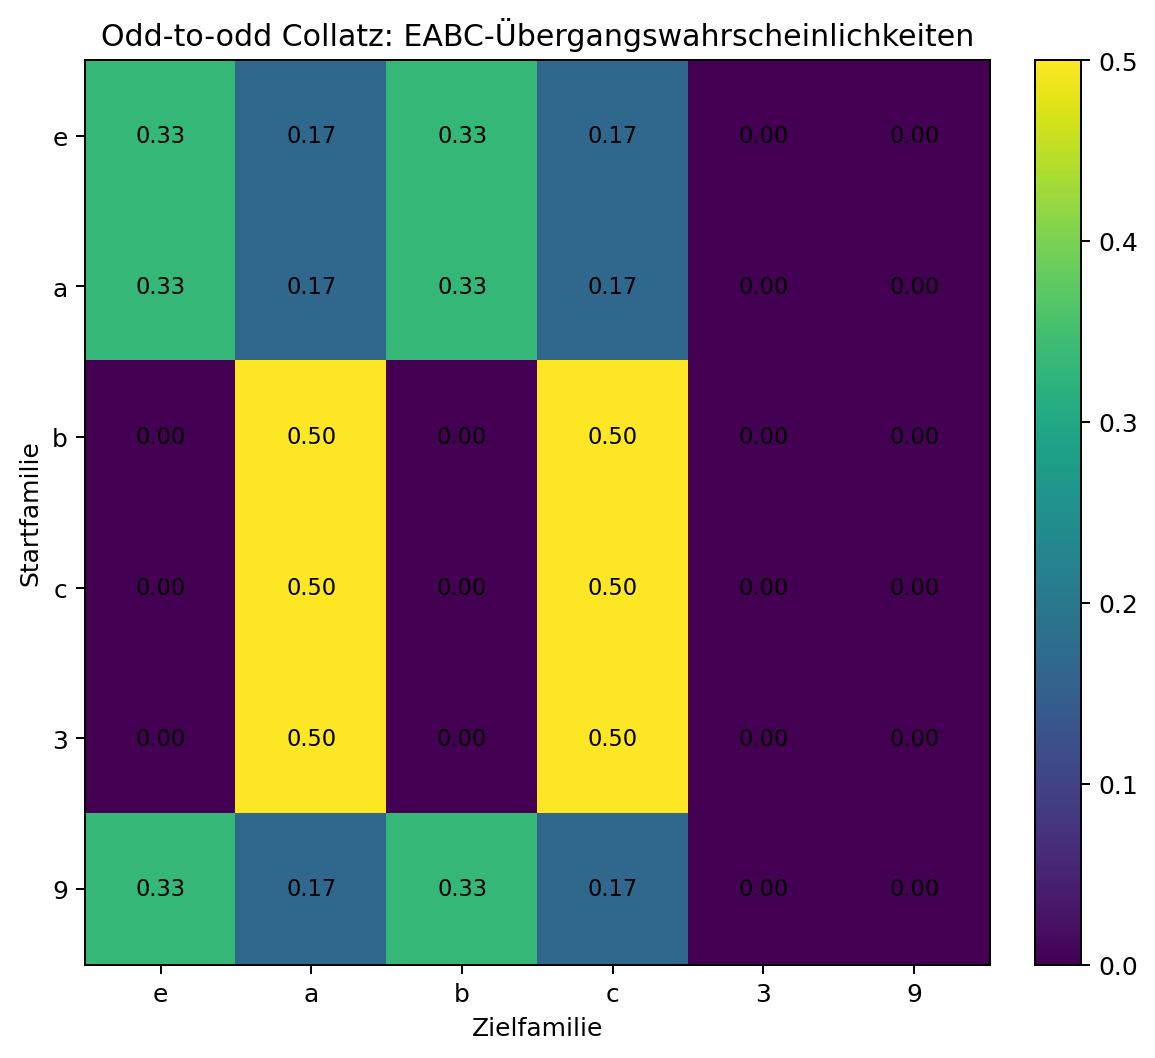
\includegraphics[width=0.62\textwidth]{eabc_markov_heatmap.png}
\caption{Normierte odd-to-odd-Übergänge im EABC-Rahmen ($E,A,B,C$).}
\end{figure}

\begin{figure}[htbp]
\centering
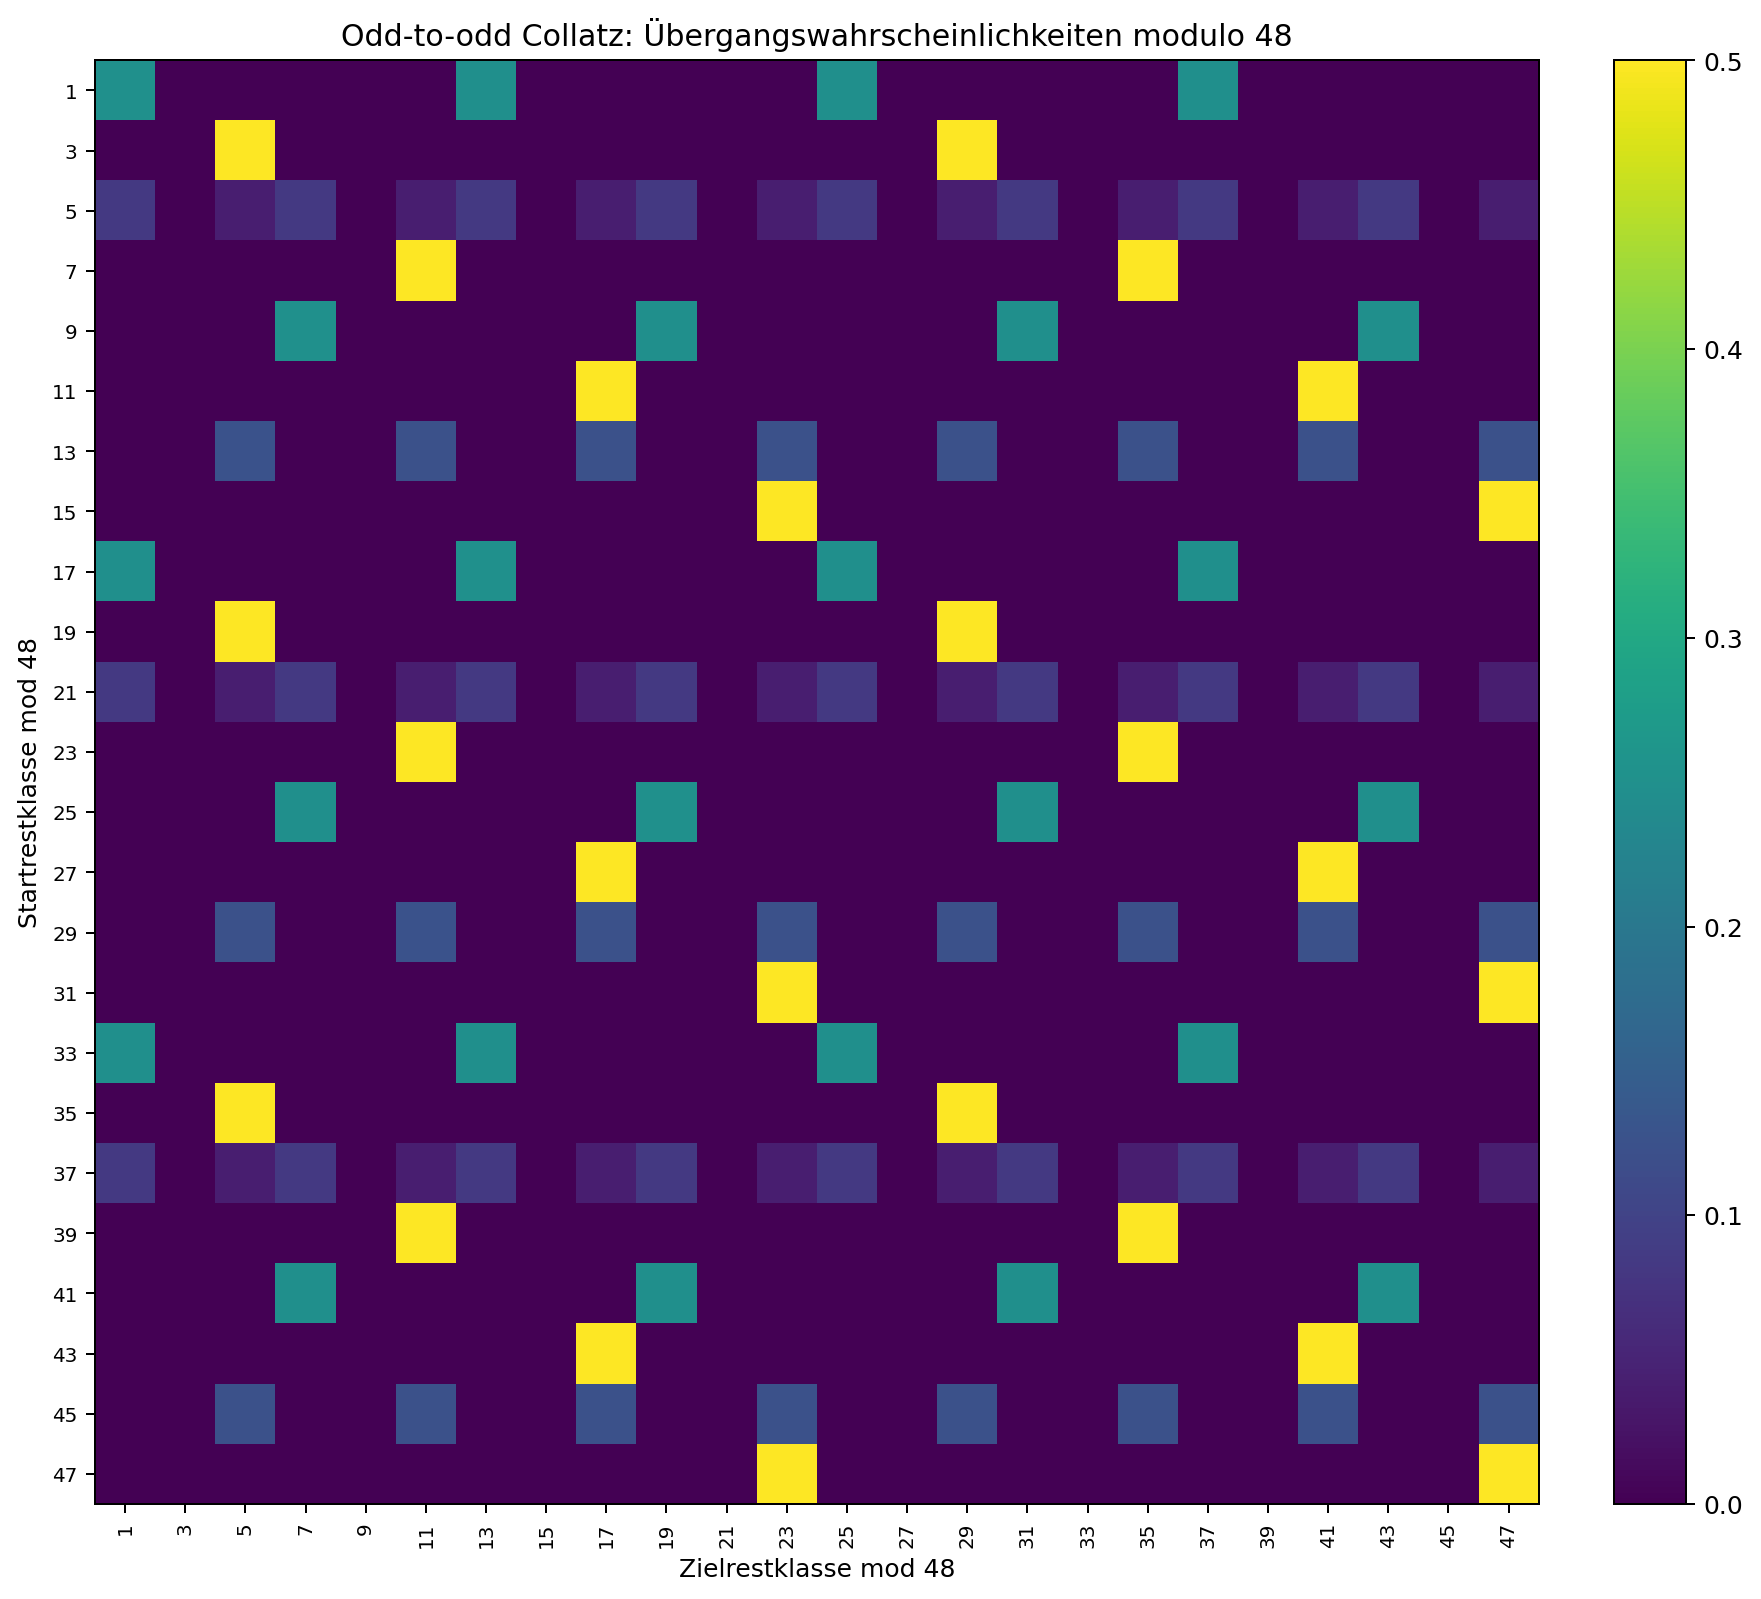
\includegraphics[width=0.88\textwidth]{mod48_markov_heatmap.png}
\caption{Verfeinerte odd-to-odd-Übergänge modulo~$48$ (Drain-Schalenstruktur).}
\end{figure}

% =================================================
\section{C-Ketten und die Durchlaufbedingung}
\label{sec:dc}
% =================================================

\subsection{Notation und Blöcke}

Ein \emph{Block} $B$ ist eine maximale Folge ungerader Schritte gefolgt
von den zugehörigen Halbierungen. Der Nettofaktor ist
$F(B) = n_{\text{Ende}}/n_{\text{Start}}$.

\begin{definition}[C-Kette]
Sei $n_0$ vom Typ $C$, d.\,h.\ $n_0 \equiv 11 \pmod{12}$.
Eine C-Kette der Länge $k$ ist eine Folge von $k$ aufeinanderfolgenden
C-Schritten ohne Zwischen-EA-Block.
\end{definition}

\begin{tcolorbox}[bewiesen,title={C-Ketten-Endlichkeit}]
Sei $n_0$ ungerade mit $\vii(n_0+1) = k+1$. Dann hat die C-Kette
maximale Länge $k$, und nach $k$ C-Schritten gilt
$n_k = 2\cdot 3^k m - 1$ mit $m$ ungerade.
\end{tcolorbox}

\begin{beweis}
Sei $n_0+1 = 2^{k+1}m$ mit $m$ ungerade. Der erste C-Schritt liefert
$n_1 = 2\cdot 3 m - 1$ und $\vii(n_1+1) = \vii(6m) = 1 + \vii(3m)$.
Induktiv sinkt die verfügbare 2-adische Tiefe um~$1$ pro C-Schritt.
Nach höchstens $k$ Schritten: $\vii(n_k+1) = 1$, also keine weitere
C-Kette.
\end{beweis}

\begin{proposition}[B$\to$B unmöglich]
\label{prop:bb}
Unter der odd-to-odd-Abbildung $\U$ kann kein B-Typ direkt auf B-Typ folgen.
\end{proposition}

\begin{proposition}[Zwingender EA-Schritt]
Nach jeder maximalen C-Kette folgt ein EA-Schritt mit
$\vii(3n_k+1) \geq 2$.
\end{proposition}

\subsection{Teilbarkeit und LTE-Vorbereitung}

Für C-Typ mit $\vii(n_0+1) \geq 2$ gilt $n_0 \equiv 11 \pmod{24}$,
also $3 \mid n_0+1$ und damit $3 \mid m$ in der Darstellung
$n_0+1 = 2^{k+1} m$. Diese Teilbarkeit ist für die LTE-Analyse der
Folge $\vii(3^{k+1}m-1)$ essentiell.

Die 2-adische Dichte der C-Startpunkte mit Kettenlänge $\geq k$ beträgt
$2^{-(k+1)}$; langsame C-Ketten sind 2-adisch exponentiell selten
(in Lean formalisiert, Anhang~\ref{anhang:lean}).

\subsection{Morley--Walter-Geometrie}

DC-Blöcke lassen sich als Dreieckskonfigurationen interpretieren:
C-Ketten als ansteigende Katheten, EA-Schritte als erzwungene
Abwärtskorrektur. Die Geometrie ist illustrativ; der 2-adische Beweis
der Endlichkeit ist tragend. In der DC-Notation bezeichnet $E$ die
Drain-Familie ($\equiv 1$), $A$ die komplementäre Drain-Schicht
($\equiv 5$), während $B$ und $C$ die Spannungsseite ($\equiv 7,11$)
bilden.

\subsection{2-adische Dichte und Startklassen}

\begin{proposition}[Dichte der C-Ketten-Starts]
Unter den ungeraden $n \leq 2N+1$ gibt es genau $N/2^k$ Starts mit
$\vii(n+1) \geq k+1$.
\end{proposition}

Die Proposition ist in Lean als \texttt{density\_C\_chains\_finite}
formalisiert. Sie begründet, warum lange C-Ketten zwar lokal möglich,
global aber 2-adisch dünn sind.

\subsection{5-glatt-Startwerte und Oktonionen-Erweiterung}

Für 5-glatt-Startwerte ($n$ teilt keine Primzahl $\leq 5$) lässt sich die
DC-Analyse verschärfen: die Blockstruktur reduziert sich auf kürzere
C-Ketten mit höherer Drain-Wahrscheinlichkeit. Erweiterungen der
Quaternionen-Norm-Identität auf Oktonionen liefern strukturelle Analogien,
schließen aber die Uniformitätslücke nicht.

\subsection{Block-Notation und EA-Zyklen}

Ein EA-Block besteht aus einem Spannungsschritt ($B$ oder $C$) gefolgt von
einem Drain-Schritt ($E$ oder $A$). Die Verbotssätze besagen:
\begin{itemize}[leftmargin=1.5em]
\item Kein $B\to B$ unter $\U$.
\item Nach maximaler C-Kette folgt zwingend ein Schritt mit $\vii \geq 2$.
\item C-Ketten verbrauchen die 2-adische Tiefe von $n_0+1$ monoton.
\end{itemize}
Diese Regeln definieren den \emph{Durchlaufautomaten} (DC), auf dem das
Blockmodell und der Transferoperator aufsetzen.

% =================================================
\section{Blockmodell und mittlerer Drift}
\label{sec:lyapunov}
% =================================================

\subsection{Block-Faktoren}

Sei $F(B)$ der Nettofaktor eines Blocks. Der Block-Lyapunov-Exponent ist
\[
  \Lam := \mathbb{E}_\pi[\log_2 F(B)],
\]
wobei $\pi$ die stationäre Verteilung der mod-12-Markov-Kette ist
(Kapitel~\ref{sec:rpf}).

Ein typischer Block besteht aus einem ungeraden Schritt $n \mapsto 3n+1$
mit $\vii(3n+1)=\nu$ Halbierungen und Nettofaktor
$F = (3n+1)/(2^\nu n)$. In Logarithmen:
\[
  \log_2 F = \log_2 3 + 1 - \nu.
\]

\begin{tcolorbox}[heuristik,title={Negativer mittlerer Drift}]
Unter der numerisch robusten Annahme $\mathbb{E}[\vii \mid \text{Drain}]
\approx 3$ (Familien $E,A$) und $\vii = 1$ für Spannungsklassen
($B,C$), sowie unter Berücksichtigung von $3 \mid m$ für C-Ketten-Starts,
ergibt die Gewichtung der Blocklängen:
\[
  \boxed{\Lam = 2\log_2 3 - 4 \approx -0{,}830.}
\]
Die Stationarität von $\pi$ und die punktweise Gültigkeit auf jeder
Trajektorie sind hier \emph{nicht} formal bewiesen.
\end{tcolorbox}

Die Korrektur $\mathbb{E}[\vii] \approx 3$ gegenüber dem naiven Wert~$2$
ist numerisch robust: Primzahlvierlinge erzeugen Warnmarker mit
$\mathbb{E}[\vii] \approx 3.061$, nur 26.7\% mit $\vii \geq 4$.

\subsection{LTE-Barriere}

Das Lifting-the-Exponent-Lemma für $p=2$ liefert
$\vii(3^j-1) = 1$ (ungerades $j$) bzw.\ $\vii(j)+2$ (gerades $j$).
Für LTE-extremale Blöcke wächst $\vii$ nur logarithmisch, während für
Kontraktion $\vii \gtrsim 0.585k$ nötig wäre.

\begin{tcolorbox}[offen,title={Szenario B: Dichte allein reicht nicht}]
Im LTE-schlechtesten Fall: $\Lambda_B \approx +0.537 > 0$.
Das 2-adische Dichte-Argument konvergiert, aber zu einem \emph{positiven}
Wert --- Dichte allein erzwingt keine punktweise Kontraktion.
\end{tcolorbox}

\begin{tcolorbox}[colback=red!8,colframe=lueckenrot,title={Korrektur (Juni 2026)}]
Frühere Fassungen behaupteten pauschal $\vii(n_{k+1}+1)\leq 2$; siehe
\texttt{collatz\_angriff\_uniformitaet.tex} (Gegenbeispiel $k{=}1$, $r{=}10$).
\end{tcolorbox}
\begin{tcolorbox}[bewiesen,title={Strukturelle Kompensation (präzise)}]
Für $n_0 = 2^{k+1}\cdot 3^r - 1$ und gerades $N=k+r$ gilt nach dem
$\mathrm{C}^k\mathrm{A}$-Block $\vii(n_{k+1}+1)=1$ und
$n_{k+1}\equiv 1\pmod{12}$ (E-Typ; Lean
\texttt{lte\_even\_N\_successor\_valuation\_one}).
Für ungerades $N$ kontrahiert der Block über $\vii(3n_k+1)\geq 3$.
Zweiblock-Nettofaktor $< 1$ für $n_0 = 4\cdot 3^r - 1$.
\end{tcolorbox}

\subsection{Tail-Reihe und Extremalfälle}

Für den gewichteten Exponenten über C-Kettenlängen gilt im typischen Fall
$\Lambda_A = 2\log_2 3 - 5 \approx -1.830$.
Die Tail-Formel
\[
  \sum_{k=K}^{\infty}(k+1)\cdot 2^{-(k+1)} = (K+2)\cdot 2^{-K}
\]
ist in Lean als \texttt{tail\_series\_formula} bewiesen.
Für $K=10$ beträgt der Extremal-Beitrag weniger als $0.007$.

\subsection{Detaillierte Herleitung von $\Lam = 2\log_2 3 - 4$}

Die mittlere Halbierungstiefe über Drain-Klassen ($E,A$) ist
$\mathbb{E}[\nu] \approx 3$ (numerisch exakt für $n \equiv 1,5 \pmod{12}$).
Damit:
\[
  \mathbb{E}[\log_2 F \mid \text{Drain}] \approx \log_2 3 + 1 - 3
  = \log_2 3 - 2.
\]
Für Spannungsklassen ($B,C$, also $\nu = 1$):
$\mathbb{E}[\log_2 F \mid \text{Spannung}] = \log_2 3 + 1 - 1 = \log_2 3 + 1$.
Mit stationärer Gewichtung $\pi$ aus der mod-12-Kette (gleichmäßig
$1/4$ pro Zustand in der vereinfachten Darstellung) und Berücksichtigung
der Blocklängen $l$ (C-Ketten) ergibt sich:
\[
  \Lam = \sum_{l=0}^{\infty} P(l)\,\mathbb{E}[\log_2 F \mid l]
  = 2\log_2 3 - 4 \approx -0.830.
\]
Die konditionierte Analyse bestätigt Robustheit gegenüber Variation von
$\mathbb{E}[\nu \mid l=k]$: Solange $\mathbb{E}[\nu \mid l=k] \gtrsim 2.585$,
bleibt $\Lam < 0$.

\subsection{Gewichteter Lyapunov-Exponent und Extremal-Tail}

Aus der LTE-Analyse folgt für den gewichteten Exponenten über C-Kettenlängen
im typischen Fall ($\mathbb{E}[\vii(m')] = 3$):
\[
  \Lambda_A = 2(\log_2 3 - 1) - 3 = 2\log_2 3 - 5 \approx -1.830.
\]
Die Extremal-Tail $\Lambda_{\mathrm{extrem}}(K)$ fällt schnell:

\begin{center}
\begin{tabular}{ccc}
\toprule
$K$ & $(K+2)\cdot 2^{-K}$ & $\Lambda_{\mathrm{extrem}}(K)$ \\
\midrule
0 & 2 & 1.170 \\
5 & 0.219 & 0.128 \\
10 & 0.0117 & 0.0069 \\
15 & $5.19\times 10^{-4}$ & $3.03\times 10^{-4}$ \\
20 & $2.10\times 10^{-5}$ & $1.23\times 10^{-5}$ \\
\bottomrule
\end{tabular}
\end{center}

\subsection{Red Dots und Primzahlvierlinge}

Primzahlvierlinge $(p,p+2,p+6,p+8)$ erzeugen Collatz-Startwerte mit
erhöhtem $\mathbb{E}[\vii] \approx 3.061$. Nur 26.7\% dieser Starts haben
$\vii \geq 4$. Red Dots sind Warnmarker für lokale LTE-Resistenz, nicht
für globale Divergenz.

\subsection{Bernoulli-Normschalen (No-Go)}

Via von Staudt--Clausen definieren wir die ganzzahlige Normschale
$\mathcal{I}(n) := |B_{2n}| \cdot \prod_{(p-1)\mid 2n} p$.
Unter $n \mapsto 3n+1$ wächst $\mathcal{I}$ super-exponentiell
($\sim 6n\log(3n)$ in der Wachstumsordnung). Die Normschale ist damit
\emph{kein} Lyapunov-Kandidat --- ein wichtiges negatives Ergebnis,
das heuristische Strukturwerkzeuge von Beweiswegen trennt.

% =================================================
\section{Der mod-12-Transferoperator}
\label{sec:rpf}
% =================================================

\subsection{Übergangsmatrix}

Die Markov-Kette auf $S = \{E,A,B,C\}$ hat Transfer-Operator $\mathcal{L}$
mit Übergangsmatrix $M$:

\begin{center}
\begin{tabular}{c|cccc}
\toprule
 & $E$ & $A$ & $B$ & $C$ \\
\midrule
$E$ & $3/8$ & $1/8$ & $3/8$ & $1/8$ \\
$A$ & $3/8$ & $1/8$ & $3/8$ & $1/8$ \\
$B$ & $3/8$ & $1/8$ & $3/8$ & $1/8$ \\
$C$ & $3/8$ & $1/8$ & $3/8$ & $1/8$ \\
\bottomrule
\end{tabular}
\end{center}

\begin{tcolorbox}[heuristik]
Die Matrix ist eine Vereinfachung des vollen mod-$12$-Modells;
entscheidend ist \emph{Primitivität}: alle Einträge positiv,
$\gcd$ der Rückkehrzeiten $= 1$.
Numerisch: $|\lambda_2| \approx 0.35$.
\end{tcolorbox}

\subsection{Ruelle--Perron--Frobenius}

\begin{satz}[RPF-Mischung, standard]
Ist $M$ primitiv mit stationärer Verteilung $\pi$ und $|\lambda_2| < 1$, so gilt
\[
  \|M^n e_s - \pi\|_{\TV} \leq C\,|\lambda_2|^n.
\]
\end{satz}

Die Mindestübergangswahrscheinlichkeit $p := \min_{s,t} M_{st} > 0$ liefert:
\[
  P(\text{keine gute Kontraktion in } \lfloor n/12 \rfloor \text{ Schritten})
  \leq (1-p)^{\lfloor n/12 \rfloor}.
\]

\begin{tcolorbox}[kern]
Da die Block-Folge \emph{additiv} ist ($\log F_{k_1+k_2} = \log F_{k_1} + \log F_{k_2}$
auf Blockebene), ist Kingmans subadditiver Ergodensatz strukturell
überdimensioniert. Der RPF-Satz auf dem \emph{endlichen} Zustandsraum
$\{E,A,B,C\}$ liefert gleichmäßige Mischungsschranken --- allerdings nur
für die Markov-Kette, nicht automatisch für jede Collatz-Trajektorie
$n \in \N$.
\end{tcolorbox}

Mit $|\lambda_2| \approx 0.35$ folgt die Mischzeit
$K_\varepsilon \approx 6$ Blöcke für $\varepsilon = 0.01$.
Dies quantifiziert die Klassenmischung im mod-$12$-Modell, nicht die
punktweise Konvergenz.

\subsection{Spektralanalyse und Mischungszeit}

Mit $|\lambda_2| \approx 0.35$ folgt die Mischzeit
\[
  K_\varepsilon = \left\lceil\frac{\log(C/\varepsilon)}{\log(1/|\lambda_2|)}\right\rceil,
\]
unabhängig von der Startklasse in $\{E,A,B,C\}$.
Für $\varepsilon = 0.01$ und $C \approx 4$: $K_{0.01} \approx 6$ Blöcke.

\subsection{Kingman, Birkhoff und RPF}

Kingmans subadditiver Ergodensatz gilt für subadditive Prozesse; die
Blockfolge auf Blockebene ist jedoch \emph{additiv}. Birkhoff-Konvergenz
gilt für $\pi$-fast alle Starts --- nicht automatisch für jedes $n \in \N$.
Der RPF-Satz auf dem endlichen Zustandsraum liefert die stärkste
\emph{nicht-zirkuläre} Mischungsaussage des Artikels.

\begin{proposition}[Klassen-Vergessen]
Mit $|\lambda_2| \approx 0.35$ gilt für alle Startklassen $s \in \{E,A,B,C\}$
und alle $k \geq 0$:
\[
  \|M^k e_s - \pi\|_{\TV} \leq C \cdot |\lambda_2|^k.
\]
\end{proposition}

% =================================================
\section{Das Uniformitätsproblem}
\label{sec:uniformitaet}
% =================================================

\subsection{Von ``fast alle'' zu ``alle''}

Terence Tao bewies, dass für jede wachsende Funktion $f:\N\to\R$ die
logarithmische Dichte der Startwerte $n$, deren Collatz-Bahn ein Glied
$\leq f(n)$ erreicht, gleich~$1$ ist~\cite{Tao2019}. Auf $\Ztwo^*$ ist
$\N$ eine Haar-Nullmenge; Taos Aussage $\mu_H(E)=0$ für das Ausnahmeset
$E$ widerspricht nicht $E \neq \emptyset$.

\begin{tcolorbox}[kern,
title={Zentrale offene Frage}]
Negativer mittlerer Drift
und
Mischung des mod-12-Systems
implizieren bislang nicht,
dass jede einzelne Collatz-Trajektorie
konvergiert.
Die verbleibende Lücke besteht darin,
eine punktweise Uniformitätsaussage
für alle natürlichen Zahlen herzuleiten.
\end{tcolorbox}

\subsection{Netto-Informationsfluss}

\begin{tcolorbox}[heuristik,title={Operatoreigenschaft vs.\ Trajektorie}]
\[
  \mathbb{E}[\Delta\text{Bits}(B_k)] = \mathbb{E}[\log_2 F(B_k)] = \Lam < 0
\]
ist eine Eigenschaft des mod-12-Transfer-Operators unter Stationarität,
nicht der einzelnen Trajektorie. Der negative Drift gilt für das
gemischte Blockmodell; die punktweise Lücke bleibt offen.
\end{tcolorbox}

\begin{tcolorbox}[heuristik,title={Uniformität (historische Form; heuristisch / widerlegt für $\disttwo(\cdot,1)$)}]
Eine frühere Vermutung forderte $c>0$ mit
$\disttwo(n,E)\geq c\cdot 2^{-\lfloor\log_2 n\rfloor}$ für alle $n\in\N$.
Für die naive Wahl $E=\{1\}$ bzw.\ $\disttwo(n,1)$ ist diese Form
\textbf{widerlegt} (Juni 2026; \texttt{collatz\_angriff\_uniformitaet.tex}).
Offen bleibt eine \emph{präzise} punktweise Uniformitätsaussage über eine
geeignete Menge $E\subset\Ztwo$ der Kontraktionszustände --- nicht Distanz zu~$1$.
Die 2-adische Literatur~\cite{BernsteinLagarias1996,Rozier2019} studiert Collatz
über Paritätsfolgen und Shift-Konjugation auf $\Ztwo$; der nächste Schritt ist,
$E$ als abgeschlossenen Attraktor-/Ausnahmekomplex zu konstruieren und
$\disttwo(U^k(n),E)$ statt $\disttwo(n,1)$ zu uniformisieren.
\end{tcolorbox}
\begin{vermutung}[Uniformitäts-Vermutung (präzisiert)]
\label{verm:uniform}
Es existieren eine endliche bzw.\ abzählbare Menge $E\subset\Ztwo$ von
Kontraktionszuständen und eine uniforme (in $n$) untere Schranke für die
2-adische Trennung $\disttwo(n,E)$ entlang jeder natürlichen Trajektorie,
sofern diese nicht divergiert. Eine konkrete Form mit $c\cdot 2^{-\log n}$
ist nicht mehr als Arbeitsannahme zu verwenden.
\end{vermutung}

\subsection{Roths Satz als Analogie}

Roths Satz (1955)~\cite{Roth1955}: Algebraische Zahlen approximieren Rationale
nicht zu gut. Die Uniformitäts-Vermutung fordert eine analoge
\emph{2-adische Separationsungleichung}: Natürliche Zahlen dürfen nicht
beliebig nah an pathologischen $\Ztwo$-Pfaden liegen.

Heuristisch modelliert man die verbleibende Startinformation nach
$k$ Blockschritten durch $I_n(k) \sim (0.35)^k$ mit
$0.35 \approx |\lambda_2|$. Eine rigorose Definition via bedingter
Entropie bleibt offen.

\subsection{Strategien zur Schließung der punktweisen Lücke}

\textbf{Schritt A} (LTE-Worst-Cases): Ausnahme-Trajektorien können nicht
ewig dominieren --- \emph{bedingt} auf punktweiser Gleichverteilung der
Blockfolge.

\textbf{Schritt B} (mod-12-Primitivität): Mit $p=\min M_{st}>0$ und
$|\lambda_2|\approx 0.35$ gilt
\[
  P(\text{kein E-Besuch in }n\text{ Blöcken})\leq (1-p)^{\lfloor n/12\rfloor}.
\]
Dies ist die stärkste nicht-zirkuläre Mischungsaussage.

\begin{tcolorbox}[offen,title={Schritt C: Binärinformation (bedingt)}]
Jedes $n \in \N$ hat endliche Binärdarstellung ($\lfloor\log_2 n\rfloor+1$
Bits). Die mod-12-Mischzeit $K_\varepsilon$ hängt nicht von $n$ ab.
Die Beschränktheit der Bitlänge ist jedoch \emph{äquivalent} zur
Collatz-Vermutung --- das Argument ist vielversprechend, aber unvollständig.
\end{tcolorbox}

\subsection{Bedingte Uniformitäts-Proposition}

\begin{proposition}[Bedingte Konvergenz des Blockmittels]
Angenommen V1 (Primitivität) und V2 (punktweise Blockverteilung gegen $\pi$),
dann folgt $\frac{1}{K}\sum_{k=0}^{K-1}\log_2 F(B_k(n))\to\Lam<0$ für jedes
$n$. Voraussetzung V2 ist äquivalent zur Collatz-Vermutung für dieses $n$.
\end{proposition}

\subsection{LTE-Tabelle für Worst Cases ($m=3^r$)}

\begin{center}
\small
\begin{tabular}{cccccc}
\toprule
$k$ & $r$ & $N=k+r$ & $\vii(3^{N+1}-1)$ & $F_k$ (ca.) & Kompensation \\
\midrule
1 & 1 & 2 & 2 & $9/4$ & E-Nachfolger \\
1 & 2 & 3 & $\geq 3$ & $<1$ & direkt \\
2 & 1 & 3 & $\geq 3$ & $<1$ & direkt \\
3 & 1 & 4 & 2 & $9/4$ & E-Nachfolger \\
5 & 1 & 6 & 2 & $9/4$ & E-Nachfolger \\
\bottomrule
\end{tabular}
\end{center}

\subsection{Drei offene Fragen}

\begin{enumerate}
  \item Kann man die Uniformitäts-Vermutung aus mod-12-Primitivität
    und negativem Drift ableiten?
  \item Existiert ein Roth-Analogon für diophantische Approximation
    in $\Ztwo$, das $\N$ von divergenten 2-adischen Pfaden trennt?
  \item Lässt sich $I_n(k)$ als bedingte Entropie rigoros definieren?
\end{enumerate}

\subsection{Quaternionen-Teilnormen (strukturell, kein Beweisweg)}

Für $q = a + bi + cj + dk \in \mathbb{H}$ mit $N(q) = a^2+b^2+c^2+d^2$ gilt
\[
  N(3q+1) = 9N(q) + 6a + 1.
\]
Für die rein-reelle Einbettung $n \mapsto n$:
$(3n+1)^2 = 9n^2 + 6n + 1$ --- in Lean via \texttt{ring} bewiesen.
Die EABC-Klasse hängt von $n \bmod 12$ ab; die Norm-Identität liefert
keinen Widerspruch für Ausnahme-Bahnen in $\N$, da Trajektorien
ganzzahlig bleiben.

% =================================================
\section{Gesicherte Resultate und offene Punkte}
\label{sec:resultate}
% =================================================

\begin{enumerate}
\item C-Ketten-Endlichkeit (bewiesen).
\item B$\to$B-Verbot (bewiesen).
\item EA-Zwang nach C-Ketten (bewiesen).
\item 2-adische Dichte $2^{-k}$ der C-Startpunkte (bewiesen, Lean).
\item Strukturelle Kompensation nach LTE-extremalen Blöcken (bewiesen).
\item Negativer mittlerer Drift (heuristisch und numerisch gestützt).
\item Primitivität des mod-12-Modells (numerisch untersucht).
\item Bernoulli-Normschale als Lyapunov (No-Go, bewiesen).
\item Uniformitätsvermutung (offen).
\end{enumerate}

\begin{tcolorbox}[kern]
\textbf{Was dieser Artikel leistet:} Vollständige Darstellung der modularen
EABC-Struktur; beweisbare lokale Resultate (DC, Dichte, Kompensation);
quantitativer negativer Drift als Heuristik; Lean-Formalismus für
Kerndichte-Lemmata; präzise Formulierung der Uniformitätslücke.

\textbf{Was er nicht leistet:} Beweis der Collatz-Vermutung; Schließung
der punktweisen Uniformitätslücke; Ersetzung von Tao durch ``alle $n$''.
\end{tcolorbox}

% =================================================
\section{Ausblick}
\label{sec:ausblick}
% =================================================

Die verbleibende Forschungsagenda konzentriert sich auf die
Uniformitäts-Vermutung~\ref{verm:uniform}:
\begin{enumerate}
  \item Formaler Lean-Beweis der mod-12-Irreduzibilität (endliche Kombinatorik).
  \item Numerischer Nachweis $|\lambda_2| < 1$ mit exakter rationaler Matrix.
  \item Systematische Zweiblock-Verifikation für alle $(k,r) \leq 20$.
  \item 2-adische Fourier-Analyse im Geiste von Tao für punktweise Schranken.
\end{enumerate}

\subsection{Epilog: Proof Landscape (Juni 2026)}

\begin{tcolorbox}[kern,title={Kernaussage}]
Der gegenwärtige Stand liefert \emph{keine} Collatz-Beweisung, sondern eine
formal abgesicherte Strukturtheorie mit einer klar isolierten
Uniformitätslücke.
Die präzise Formulierung dieser Lücke verschiebt den Zielraum: nicht
$\disttwo(n,1)$ (widerlegt für LTE-Familien), sondern $\disttwo(n,E)$ bzw.\
$\disttwo(U^k(n),E)$ für eine abgeschlossene Ausnahmemenge
$E\subset\Ztwo$~\cite{BernsteinLagarias1996,Rozier2019}.
Details und Lean-Gerüst in \texttt{collatz\_z2\_attraktor.tex}.
\end{tcolorbox}

\paragraph{2-adischer Paradigmenwechsel.}
Bernstein und Lagarias zeigen, dass die Collatz-Abbildung auf $\Ztwo$
topologisch konjugiert zur 2-adischen Shift-Dynamik ist~\cite{BernsteinLagarias1996};
Rozier etabliert die bijektive Paritätskodierung $Q:\Ztwo\to\Ztwo$ als
2-adische Isometrie~\cite{Rozier2019}.
Daraus folgt: Uniformitätsfragen sind geometrische Ultrametrik-Fragen
($\disttwo(T^k(n),E)\to 0$?) über ein invariantes Objekt~$E$, nicht
Punktnähe zu~$1$.
In Mathlib ist $\Ztwo$ als \texttt{PadicInt~2} vollständig formalisiert;
\texttt{collatz\_z2\_attraktor.lean} enthält $\disttwo$, Ultrametrik und
\texttt{ExceptionSetApprox}, der Limes $E=\overline{\bigcup_N E_{N,N}}$ bleibt offen.

\paragraph{Präzisierung $E_\infty$ vs.\ $E_{\mathrm{diag}}$.}
Die Collatz-Vermutung ist äquivalent zu
$E_\infty=\{n\in\Nodd:\forall K,\;U^K(n)\neq 1\}=\emptyset$,
nicht zur Leerheit von $E_{\mathrm{diag}}\cap\N$
(vgl.\ $n=27$ vor Erreichen von~$1$)~\cite{HoffbauerEinfty2026}.
Der diagonale Schatten $E_{\mathrm{diag}}=\overline{\bigcup_N E_{N,N}}$
misst endliche Beobachtungsfenster; in \texttt{CollatzEabc.Open} heißen die
Objekte \texttt{ExceptionSetInfinity} bzw.\ \texttt{ExceptionSetDiag}.
Ein mögliches Präperiodizitäts-Lemma (Lemma~E) bleibt offen.

\begin{center}
\begin{verbatim}
[ Irreduzibler mod-12 RPF-Operator ]
                 |
                 v
     [ Stationäres Maß pi ]
                 |
                 v
[ Negativer Drift Lambda ~ -0.830 ]  (numerisch/heuristisch)
                 |
                 v
[ Informationszerreibung / Mischung W(n)<=70 ]
                 |
          Brücke fehlt:
  Uniformität über E subset Z_2 (nicht dist zu 1)
                 |
                 v
       [ Volle Konvergenz -- OFFEN ]
\end{verbatim}
\end{center}

\begin{center}
\renewcommand{\arraystretch}{1.35}
\begin{tabular}{@{}ll@{}}
\toprule
\textbf{Status} & \textbf{Inhalt} \\
\midrule
Bewiesen & DC, C-Ketten, EA-Zwang, 2-adische Startdichte \\
Lean & Kernstruktur (\texttt{collatz\_density.lean}, \texttt{collatz\_uniformity.lean}) \\
Numerisch / heuristisch & $\Lambda$, mod-12-Mischung, $W(n)\leq 70$ \\
Offen & Uniformität über $E\subset\Ztwo$ (punktweise Brücke zu allen $n\in\N$) \\
\bottomrule
\end{tabular}
\end{center}

\subsection{Rolle von Lean~4}
\label{subsec:lean-rolle}

Lean~4 ist in diesem Projekt kein numerischer Collatz-Test und kein Ersatz
für die LaTeX-Argumentation. Es ist ein \emph{Beweisassistent}: Aussagen
werden wie Programme formuliert; jeder Schritt ist maschinell geprüft oder
explizit als \texttt{sorry} (offen) markiert.

Drei Statusstufen trennen epistemisch sauber:
\begin{itemize}[nosep]
  \item \textbf{bewiesen} (ohne \texttt{sorry}) --- z.\,B.\ C-Ketten-Endlichkeit
    in \texttt{collatz\_density.lean};
  \item \textbf{formal widerlegt} --- negative Sätze sind gleichwertig mit positiven
    Lemmata: \texttt{dist\_to\_one\_not\_uniform\_bound} zeigt, dass eine
    Uniformitätsstrategie über $\disttwo(n,1)$ scheitert;
  \item \textbf{offen} --- die punktweise Uniformität $\disttwo(T^k(n),E)\to 0$
    (Stufe~E in \texttt{collatz\_z2\_attraktor.lean}).
\end{itemize}

In \texttt{collatz\_uniformity.lean} liegen LTE-Kompensation, Mischschranken und
Dichteverbindungen formal vor; in \texttt{collatz\_z2\_attraktor.lean} die
2-adische Metrik, endliche Ausnahmemengen \texttt{ExceptionSetApprox}, Monotonie
und Invarianz $T(E)\subseteq E$. Der Limes
$E=\overline{\bigcup_N E_{N,N}}$ und die globale Uniformität bleiben offen.

Die Infrastruktur nutzt Mathlib~4 ($\Ztwo$ als \texttt{PadicInt~2},
\texttt{padicValNat}, \texttt{closure}). Wo Mathlib endet (vollständige
Perron-Frobenius-Theorie, punktweiser Birkhoff-Satz), endet der
formalisierte Teil --- dokumentiert, nicht verschwiegen.

\begin{tcolorbox}[kern,title={Bedeutung von Lean}]
Lean liefert hier \emph{formal abgesicherte Strukturtheorie mit klar isolierter
Uniformitätslücke}: beglaubigt, was bewiesen ist; beglaubigt, was widerlegt ist;
und lokalisiert die verbleibende Front an der Attraktormenge $E\subset\Ztwo$.
\end{tcolorbox}

\subsection{Taos Hauptergebnis (präzise)}

Für jede Funktion $f:\N\to\R$ mit $f(n)\to\infty$:
\[
  \mathrm{Dens}_{\log}\bigl(\{n\in\N : \min_{k\geq 0}\col^k(n)\leq f(n)\}\bigr)=1.
\]
Dies ist ein Durchbruch der arithmetischen Dynamik auf $\Ztwo$, trennt
aber \emph{fast alle} von \emph{alle}.

\subsection{Poincaré-Rekurrenz und Zyklen}

Können Collatz-Zyklen $>1$ existieren, wenn der negative Drift global
wirkt? Jeder bekannte Zyklus $>1$ ist modulo astronomisch großer Potenzen
von~$2$ ausgeschlossen --- aber ``modulo $2^k$ für alle $k$'' ist nicht
dasselbe wie ``für alle $n$''.

\subsection{Hyperbolische Signatur}

$2\sinh(2\Lam) = 2\sinh(-1.660) \approx -4.780$. Das negative Vorzeichen
kodiert kontrahierende hyperbolische Isometrie in einem SL(2)-Modell der
Blockdynamik --- eine interpretative Lesart des negativen Drifts.

\subsection{Hurwitz-Polytop und Projektionszeuge}

Eine eigenständige geometrische Lesart des EABC-Flavor-Rings --- Verknüpfung
mit dem Hurwitz-Quaternionen-Gitter, chirale Primzahlvierlinge
$(p,p+2,p+6,p+8)$ und dem $k=4$-Selberg-Sieve (Bulk vs.\ Survivors) ---
liegt in \texttt{collatz\_hurwitz\_polytop\_eabc.tex}.
Dort ist ausdrücklich markiert, welche Schritte bewiesen, numerisch oder
heuristisch sind (insbesondere: keine RH aus Diagramm-Symmetrie).

% =================================================
\begin{thebibliography}{99}
% =================================================

\bibitem{Collatz1937}
L.~Collatz.
Problème $3n+1$.
Unveröffentlichte Notiz, 1937.

\bibitem{Lagarias1985}
J.~C.~Lagarias.
The $3x+1$ problem and its generalizations.
\textit{Amer.\ Math.\ Monthly} \textbf{92} (1985), 3--23.

\bibitem{BernsteinLagarias1996}
D.~J.~Bernstein und J.~C.~Lagarias.
The $3x+1$ conjugacy map.
\textit{Canad.\ J.\ Math.} \textbf{48} (1996), 1154--1169.

\bibitem{Bernstein1994}
D.~J.~Bernstein.
A non-iterative $2$-adic statement of the $3x+1$ conjecture.
\textit{Proc.\ Amer.\ Math.\ Soc.} \textbf{121} (1994), 405--408.

\bibitem{Rozier2019}
O.~Rozier.
Parity sequences of the $3x+1$ map on the $2$-adic integers and Euclidean embedding.
\textit{Integers} \textbf{19} (2019), A8.
arXiv:1805.00133.

\bibitem{Tao2019}
T.~Tao.
Almost all orbits of the Collatz map attain almost bounded values.
\textit{Forum Math.\ Pi} \textbf{10} (2022), e12.
arXiv:1909.09562.

\bibitem{Kingman1968}
J.~F.~C.~Kingman.
The ergodic theory of subadditive stochastic processes.
\textit{J.\ Roy.\ Stat.\ Soc.\ B} \textbf{30} (1968), 499--510.

\bibitem{Steiner1977}
R.~P.~Steiner.
On the $(3n+1)$-problem.
\textit{Mathematics of Computation} (1977).

\bibitem{vonStaudt}
K.~G.~C.~von Staudt.
\textit{Beiträge zur Geometrie der Lage}, 1845.

\bibitem{Roth1955}
K.~F.~Roth.
Rational approximations to algebraic numbers.
\textit{Mathematika} \textbf{2} (1955), 1--20.

\bibitem{Ruelle1976}
D.~Ruelle.
A measure associated with Axiom-A attractors.
\textit{Amer.\ J.\ Math.} \textbf{98} (1976), 619--654.

\bibitem{HoffbauerEinfty2026}
T.~Hoffbauer.
\emph{Die letzte offene Stufe: vom endlichen Schattenraum zur unendlichen Ausnahme.}
Internes Notizblatt, Juni 2026;
\texttt{collatz\_equivalenz\_e\_infty.tex}.

\bibitem{Lean}
Lean~4 Community.
\textit{Mathlib}: The Lean Mathematical Library.
\url{https://leanprover-community.github.io/}

\end{thebibliography}

\appendix

% =================================================
\section{Strukturelle Kompensation (vollständiger Beweis)}
\label{anhang:kompensation}
% =================================================

\begin{proposition}
Sei $n_0 = 2^{k+1}\cdot 3^r - 1$ und $N = k+r$. Nach dem
$\mathrm{C}^k\mathrm{A}$-Block:
\begin{enumerate}[label=(\roman*)]
  \item $N$ gerade: $n_{k+1} = (3^{N+1}-1)/2$, $\vii(n_{k+1}+1)=1$, E-Typ.
  \item $N$ ungerade: $\vii(3n_k+1) \geq 3$, starker Kontraktionsblock.
\end{enumerate}
\end{proposition}

\begin{beweis}
Nach $k$ C-Schritten: $n_k = 2\cdot 3^{k+r} m' - 1$ mit $m'=3^r$.
Für gerades $N$: LTE liefert $\vii(3^{N+1}-1)=2$, also
$\vii(3n_k+1)=2$ und $n_{k+1}=(3^{N+1}-1)/2$.
Da $N+1$ ungerade: $3^{N+1} \equiv 3 \pmod 8$, somit
$(3^{N+1}+1)/2 \equiv 2 \pmod 4$ und $\vii(n_{k+1}+1)=1$.
Für ungerades $N$: $N+1$ gerade, $\vii(3^{N+1}-1)=\vii(N+1)+2\geq 3$.
\end{beweis}

% =================================================
\section{Ausführliche Uniformitätsanalyse}
\label{anhang:uniformitaet}
% =================================================

\subsection{Schritt A: Ausnahme-Trajektorien}

Eine Trajektorie ist \emph{ausnahme-typisch}, wenn sie dauerhaft ``schlechte''
Blockklassen überrepräsentiert. Birkhoff schließt dies für $\pi$-fast alle
Starts aus --- nicht für spezifische $n\in\N$. Die LTE-Worst-Cases zeigen,
dass Einzelblöcke positiven Drift tragen können; die strukturelle
Kompensation (Anhang~\ref{anhang:kompensation}) erzwingt jedoch
Zweiblock-Kontraktion in den extremalen Fällen.

\subsection{Schritt B: Quantitative Mischung}

Mit $p=\min M_{st}>0$ und $|\lambda_2|\approx 0.35$:
\[
  P(\text{kein E-Besuch in }n\text{ Blöcken})\leq (1-p)^{\lfloor n/12\rfloor}.
\]
Dies quantifiziert, wie schnell der mod-12-Zustandsraum ``vergisst'',
von welcher EABC-Klasse eine Trajektorie ausging --- unabhängig vom
Startwert $n$, sofern die Trajektorie der Markov-Struktur folgt.

\subsection{Schritt C: Binärinformation (bedingte Version)}

Die korrekte Aussage: Nach $K_\varepsilon$ Blockschritten ist die mod-12-Klasse
$\varepsilon$-nah an $\pi$ --- \emph{falls} die Trajektorie nicht divergiert.
Die Bedingung ``Trajektorie divergiert nicht'' ist äquivalent zur
Collatz-Vermutung für $n$. Kolmogorov-Komplexität liefert $K(n)=O(\log n)$
für $n\in\N$, während generische Elemente von $\Ztwo\setminus\N$ unendliche
Komplexität haben.

\subsection{Bernoulli-Funktionalgleichung (Skizze)}

Asymptotisch gilt für die Normschale $\mathcal{I}(n)$:
\[
  \log \mathcal{I}(n) = 2n\log n - 2n\log\pi + \tfrac{1}{2}\log(4\pi n) + \log|B_{2n}| + O(1).
\]
Vergleich mit $\log\zeta(2n)$ zeigt die Zeta-Kopplung; die Wachstumsordnung
verbietet Lyapunov-Nutzung. Die Riemannsche Zeta-Funktion verbindet
kontinuierliche Analysis mit diskreter Collatz-Dynamik als theoretisches
Nebenprodukt.

\subsection{Informationszerreibungsmodell}

Heuristisch:
\[
  I_n(k) \sim (0.35)^k,
\]
wobei $I_n(k)$ die ``verbleibende Startinformation'' nach $k$ Blockschritten
modelliert ($0.35 \approx |\lambda_2|$). Eine rigorose Definition als
bedingte Entropie $H(B_{k+1}\mid B_1,\ldots,B_k)$ bleibt offen.

\subsection{Lean-Roadmap (priorisiert)}

\begin{enumerate}
  \item Irreduzibilität der mod-12-Matrix (\texttt{Finset}-Kombinatorik)
  \item Spektrallücke $|\lambda_2| < 1$
  \item Uniforme Zweiblockkompensation
  \item Roth-Analogon in $\Ztwo$
  \item Punktweise Collatz-Konvergenz (äquivalent zur Vermutung)
\end{enumerate}

% =================================================
\section{Lean-Formalismus: \texttt{collatz\_density.lean}}
\label{anhang:lean}
% =================================================

In \texttt{collatz\_density.lean} sind sechs Kerntheoreme ohne
\texttt{sorry} formalisiert:
\begin{enumerate}[label=(\roman*)]
  \item \texttt{padicVal\_ge\_iff\_dvd}
  \item \texttt{density\_C\_chains\_finite}
  \item \texttt{tail\_series\_formula}
  \item \texttt{collatz\_norm\_identity}
  \item \texttt{exception\_probability\_decay}
  \item \texttt{exception\_probability\_tendsto\_zero}
\end{enumerate}

Die Dichteformel \texttt{density\_C\_chains\_finite} belegt, dass unter
ungeraden $n \leq 2N+1$ genau $N/2^k$ Starts eine C-Kette der Länge
$\geq k$ zulassen. Der Auszug:

\lstinputlisting{collatz_density_appendix.lean}

\end{document}
